


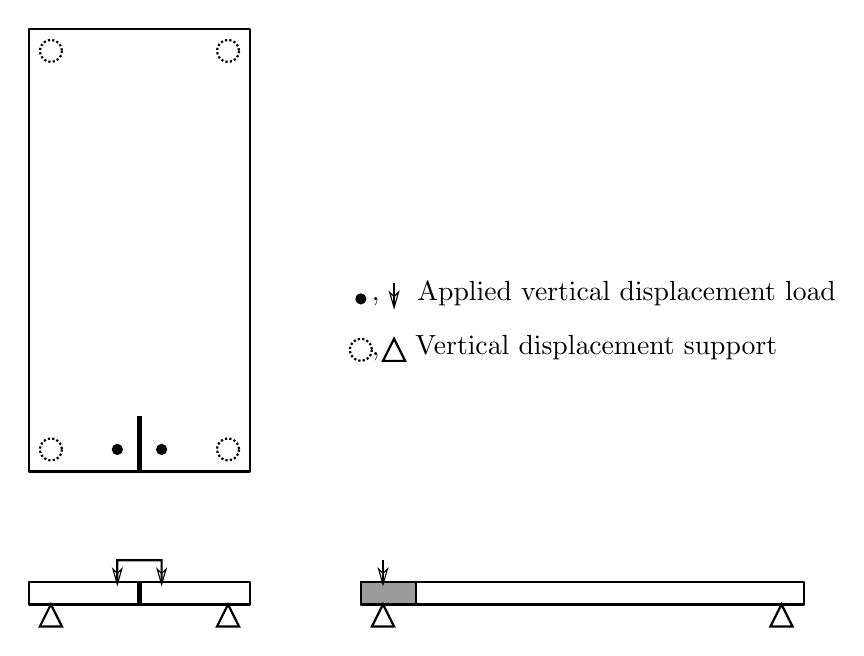
\begin{tikzpicture}[y=0.80pt, x=0.8pt,yscale=-1, inner sep=0pt, outer sep=0pt]
\begin{scope}[shift={(0,-552.36218)}]
  \path[shift={(0,552.36218)},draw=black,fill=black,line join=round,miter
    limit=4.00,fill opacity=0.000,nonzero rule,line width=0.800pt,rounded
    corners=0.0000cm] (50.0000,50.0000) rectangle (150.0000,250.0000);
  \path[shift={(0,552.36218)},draw=black,fill=black,dash pattern=on 0.80pt off
    0.80pt,line join=round,miter limit=4.00,fill opacity=0.000,nonzero rule,line
    width=0.800pt]
    (65.0000,60.0000)arc(0.000:180.000:5.000)arc(-180.000:0.000:5.000) -- cycle;
  \path[shift={(0,552.36218)},draw=black,fill=black,dash pattern=on 0.80pt off
    0.80pt,line join=round,miter limit=4.00,fill opacity=0.000,nonzero rule,line
    width=0.800pt]
    (145.0000,60.0000)arc(0.000:180.000:5.000)arc(-180.000:0.000:5.000) -- cycle;
  \path[shift={(80.0,732.36218)},draw=black,fill=black,dash pattern=on 0.80pt off
    0.80pt,line join=round,miter limit=4.00,fill opacity=0.000,nonzero rule,line
    width=0.800pt]
    (65.0000,60.0000)arc(0.000:180.000:5.000)arc(-180.000:0.000:5.000) -- cycle;
  \path[shift={(0,732.36218)},draw=black,fill=black,dash pattern=on 0.80pt off
    0.80pt,line join=round,miter limit=4.00,fill opacity=0.000,nonzero rule,line
    width=0.800pt]
    (65.0000,60.0000)arc(0.000:180.000:5.000)arc(-180.000:0.000:5.000) -- cycle;
  \path[shift={(0,552.36218)},draw=black,line join=miter,line cap=butt,miter
    limit=4.00,line width=1.600pt] (100.0000,250.0000) -- (100.0000,225.0000);
  \path[draw=black,fill=black,line join=round,miter limit=4.00,fill
    opacity=0.000,nonzero rule,line width=0.800pt,rounded corners=0.0000cm]
    (50.0000,852.3622) rectangle (150.0000,862.3622);
  \path[draw=black,line join=miter,line cap=butt,miter limit=4.00,line
    width=1.600pt] (100.0000,862.3622) -- (100.0000,852.3622);
  \path[draw=black,line join=miter,line cap=butt,line width=0.800pt]
    (55.0000,872.3622) -- (60.0000,862.3622) -- (65.0000,872.3622) -- cycle;
  \path[draw=black,line join=miter,line cap=butt,line width=0.800pt]
    (135.0000,872.3622) -- (140.0000,862.3622) -- (145.0000,872.3622) -- cycle;
    \path[color=black,fill=black,line width=0.800pt] (89.5000,841.8750) --
      (89.5000,842.3750) -- (89.5000,852.3750) -- (90.5000,852.3750) --
      (90.5000,842.8750) -- (109.5000,842.8750) -- (109.5000,852.3750) --
      (110.5000,852.3750) -- (110.5000,842.3750) -- (110.5000,841.8750) --
      (110.0000,841.8750) -- (90.0000,841.8750) -- (89.5000,841.8750) -- cycle;
    \path[draw=black,even odd rule,line width=0.400pt] (90.0000,848.3622) --
      (88.0000,846.3622) -- (90.0000,853.3622) -- (92.0000,846.3622) --
      (90.0000,848.3622) -- cycle;
    \path[draw=black,even odd rule,line width=0.400pt] (110.0000,848.3622) --
      (108.0000,846.3622) -- (110.0000,853.3622) -- (112.0000,846.3622) --
      (110.0000,848.3622) -- cycle;
  \path[shift={(0,552.36218)},draw=black,fill=black,line join=round,miter
    limit=4.00,fill opacity=0.000,nonzero rule,line width=0.800pt,rounded
    corners=0.0000cm] (200.0000,300.0000) rectangle (400.0000,310.0000);
  \path[draw=black,line join=miter,line cap=butt,line width=0.800pt]
    (385.0000,872.3622) -- (390.0000,862.3622) -- (395.0000,872.3622) -- cycle;
  \path[draw=black,line join=miter,line cap=butt,line width=0.800pt]
    (205.0000,872.3622) -- (210.0000,862.3622) -- (215.0000,872.3622) -- cycle;
    \path[color=black,fill=black,line width=0.800pt] (209.5000,842.3622) --
      (209.5000,852.3622) -- (210.5000,852.3622) -- (210.5000,842.3622) --
      (209.5000,842.3622) -- cycle;
    \path[draw=black,even odd rule,line width=0.400pt] (210.0000,848.3622) --
      (208.0000,846.3622) -- (210.0000,853.3622) -- (212.0000,846.3622) --
      (210.0000,848.3622) -- cycle;
  \path[shift={(0,552.36218)},draw=black,fill=black,line join=round,miter
    limit=4.00,fill opacity=0.392,nonzero rule,line width=0.800pt,rounded
    corners=0.0000cm] (200.0000,300.0000) rectangle (225.0000,310.0000);
  \path[shift={(0,552.36218)},draw=black,fill=black,line join=round,miter
    limit=4.00,nonzero rule,line width=0.800pt]
    (92.0000,240.0000)arc(0.000:180.000:2.000)arc(-180.000:0.000:2.000) -- cycle;
  \path[shift={(20.0,552.36218)},draw=black,fill=black,line join=round,miter
    limit=4.00,nonzero rule,line width=0.800pt]
    (92.0000,240.0000)arc(0.000:180.000:2.000)arc(-180.000:0.000:2.000) -- cycle;
  \path[shift={(110.0,484.36218)},draw=black,fill=black,line join=round,miter
    limit=4.00,nonzero rule,line width=0.800pt]
    (92.0000,240.0000)arc(0.000:180.000:2.000)arc(-180.000:0.000:2.000) -- cycle;
    \path[color=black,fill=black,line width=0.800pt] (214.5000,717.3750) --
      (214.5000,727.3750) -- (215.5000,727.3750) -- (215.5000,717.3750) --
      (214.5000,717.3750) -- cycle;
    \path[draw=black,even odd rule,line width=0.400pt] (215.0000,723.3622) --
      (213.0000,721.3622) -- (215.0000,728.3622) -- (217.0000,721.3622) --
      (215.0000,723.3622) -- cycle;
  \path[shift={(140.0,687.36218)},draw=black,fill=black,dash pattern=on 0.80pt off
    0.80pt,line join=round,miter limit=4.00,fill opacity=0.000,nonzero rule,line
    width=0.800pt]
    (65.0000,60.0000)arc(0.000:180.000:5.000)arc(-180.000:0.000:5.000) -- cycle;
  \path[fill=black] (205,727.36218) node[above right] (text6089) {,};
  \path[fill=black] (205,752.36218) node[above right] (text6093) {,};
  \path[draw=black,line join=miter,line cap=butt,line width=0.800pt]
    (210.0000,752.3622) -- (215.0000,742.3622) -- (220.0000,752.3622) -- cycle;
  \path[shift={(0,552.36218)},fill=black] (225.53571,175.17857) node[above right]
    (text6099) {Applied vertical displacement load};
  \path[shift={(0,552.36218)},fill=black] (224.64285,199.46429) node[above right]
    (text6103) {Vertical displacement support};
\end{scope}

\end{tikzpicture}

